\documentclass[11pt]{article}

\usepackage[T1]{fontenc}
\usepackage[utf8]{inputenc}
\usepackage[a4paper,margin=1in]{geometry}

\usepackage{amsmath,amssymb,amsthm}
\usepackage{mathtools}
\usepackage{bm}
\usepackage{graphicx}
\usepackage{booktabs}
\usepackage{array}
\usepackage{multirow}
\usepackage{caption}
\usepackage{subcaption}
\usepackage[hidelinks]{hyperref}
\usepackage{microtype}
\usepackage{enumitem}
\usepackage{xcolor}
\usepackage{siunitx}
\usepackage{natbib}
\usepackage{tikz}
\usetikzlibrary{positioning, arrows.meta, fit, backgrounds, shapes.geometric}

\captionsetup{font=small,labelfont=bf}

\theoremstyle{plain}
\newtheorem{proposition}{Proposition}
\theoremstyle{definition}
\newtheorem{definition}{Definition}

\newcommand{\R}{\mathbb{R}}
\newcommand{\N}{\mathbb{N}}
\newcommand{\E}{\mathbb{E}}
\DeclareMathOperator*{\argmax}{arg\,max}
\DeclareMathOperator*{\argmin}{arg\,min}
\DeclareMathOperator*{\argtopk}{arg\,top\text{-}k}
\newcommand{\Kbar}{\bar{\mathbf{K}}}
\newcommand{\Vbar}{\bar{\mathbf{V}}}
\newcommand{\ur}{U_r}
\newcommand{\normq}{\lVert q \rVert_2}
\newcommand{\rad}{\rho_r}

\title{\textbf{Certified Block Screening for Adaptive Long-Context Attention}}
\author{Marcel \\ \small{Independent Researcher}}
\date{\today}

\begin{document}
\maketitle

\begin{abstract}
Long-context dense attention is expensive at inference time, and aggressive approximate-selection methods often fail unpredictably when the exact-attention budget is tight.
We propose a runtime adaptive-attention mechanism that partitions the KV cache into fixed-size blocks of length $b$, applies a coarse global path, and selects a small subset of $k \ll m = \lceil n/b \rceil$ blocks for exact attention using a certified upper bound on each block's best possible query--key score.
The bound is derived from a one-line Cauchy--Schwarz argument on per-block center and radius metadata, $\ur(q) = q^{\top} c_r + \normq \rad$, and we observe zero violations across every configuration probed.
On Qwen3-0.6B \citep{qwen3}, bound-screened adaptive attention achieves $1.07\times$, $1.38\times$, $2.24\times$, and $5.30\times$ prefill speedups over a dense SDPA \citep{dao2022flashattention} baseline at $4\mathrm{k}$, $8\mathrm{k}$, $16\mathrm{k}$, and $32\mathrm{k}$ context respectively, with no measurable calibration-perplexity loss.
Under tight exact budgets, certified screening degrades substantially more gracefully than naive fixed top-$k$ selection: at $k=5$, fixed top-$k$ collapses to a calibration perplexity of $5{,}689$, while bound screening holds at $33$.
We also report a negative result: coarse block screening at 64-token granularity fails single-token passkey retrieval \citep{liu2023lost}, and a multi-prototype block-summary extension does not rescue retrieval at the coarse selection resolution we use.
These findings position certified block screening as a practical runtime method for long-context efficiency, not a general retrieval architecture.
\end{abstract}

\vspace{0.5em}
\noindent\textit{Framing sentence.} This is a certified runtime screening method for long-context efficiency, not a general retrieval architecture.

% ======================================================================
\section{Introduction}
% ======================================================================

Long-context inference with dense attention scales quadratically with the KV
length $n$: each new query performs $O(n \cdot d)$ key--value operations
against the entire cache, for a prefill cost of $O(n^2 d)$. Runtime-efficient
alternatives trade exactness for structure: sliding-window locality
\citep{beltagy2020longformer, zaheer2020bigbird}, compression-based attention
\citep{wang2020linformer}, IO-aware exact kernels
\citep{dao2022flashattention}, or heuristic query-aware selection
\citep{tang2024quest, jiang2024minference, fu2024lazyllm}. Each compromise is
acceptable in its intended regime, but methods that rank blocks of keys by
an unbacked empirical summary score can degrade catastrophically when the
summary is uninformative for a given query --- a failure mode we observe
directly in \S\ref{sec:degradation}.

There is room for a method that (i) keeps the exact KV cache available, (ii)
spends cheap global compute on a coarse summary pass, and (iii) screens
which blocks deserve token-level exact attention using a \emph{certificate}
of possible relevance, not merely a heuristic estimate of it. We want the
certificate to be provably sound, inexpensive to compute and maintain
across decoding steps, and selective enough to produce a measurable shift
in selection when compared against a heuristic baseline.

We propose \emph{certified block screening}. Each KV block is summarised by
a center $c_r \in \R^{d}$ and a scalar radius $\rad \in \R_{\ge 0}$
satisfying $\|k_j - c_r\|_2 \le \rad$ for every key in the block (\S\ref{sec:cert});
a query $q$ is screened against blocks via the Cauchy--Schwarz upper bound
\[
\ur(q) \;=\; q^{\top} c_r \,+\, \normq \rad,
\]
which provably upper-bounds the best token-level score $\max_{j \in B_r} q^{\top} k_j$
inside the block. We implement the selector as a drop-in replacement inside
an existing dense model (Qwen3-0.6B \citep{qwen3}) with a shared-across-queries
gather path that lets the post-screening attention run as a single fused
kernel call (\S\ref{sec:systems}). On this model, certified screening
delivers prefill speedups that grow with context length, reaching $5.30\times$
at $32\mathrm{k}$ tokens (\S\ref{sec:latency}); calibration perplexity is
preserved within run-to-run jitter; and the selector's failure mode under
tight exact budgets is qualitatively softer than that of heuristic top-$k$
(\S\ref{sec:degradation}). We also identify a clear limitation: coarse
block selection at 64-token granularity is not sufficient for sparse
single-token retrieval (\S\ref{sec:limitations}), and we document a
negative multi-prototype experiment that demonstrates which of summary
resolution and selection resolution is the binding constraint.

\paragraph{Contributions.}
\begin{itemize}[leftmargin=1.4em,topsep=2pt,itemsep=1pt]
\item A certified runtime block-screening selector for adaptive long-context
      attention, with a one-line provable upper bound $\ur(q) = q^{\top} c_r + \normq \rad$
      and cheap per-block metadata (one center plus one scalar radius).
\item An empirical demonstration that certified screening improves graceful
      degradation under tight exact budgets and yields a growing
      latency--quality advantage over dense attention as context scales to
      $32\mathrm{k}$ tokens, while preserving calibration perplexity.
\item A careful negative-result analysis showing that coarse block screening
      at the tested granularity is insufficient for sparse single-token
      retrieval, and that simple multi-prototype extensions do not rescue
      retrieval because selection granularity, not summary granularity, is
      the limiting axis.
\end{itemize}

% ======================================================================
\section{Related Work}
% ======================================================================

\paragraph{Efficient long-context attention.}
FlashAttention \citep{dao2022flashattention} and its ROCm/AOTriton
descendants make dense attention IO-efficient but leave the $O(n^2)$
arithmetic intact. Linear-attention and compression methods
\citep{wang2020linformer} bound memory and throughput by restricting the
attention operator; they operate in a different approximation regime than
token-level exact attention. Sliding-window and block-sparse patterns
\citep{beltagy2020longformer, zaheer2020bigbird} hard-code a locality prior,
which is orthogonal to the runtime-selective problem we address.

\paragraph{Query-aware selective KV retrieval.}
The most directly related prior work screens or routes KV information at
inference time using query-dependent signals. Quest \citep{tang2024quest}
maintains per-page element-wise minimum and maximum key values and scores
each page against those bounds. MInference \citep{jiang2024minference}
routes queries to structured sparsity patterns selected offline.
LazyLLM \citep{fu2024lazyllm} defers and prunes KV cache tokens using
importance heuristics derived from past attention scores. SeerAttention
\citep{gao2024seer} learns intrinsic block-level sparsity inside the
attention map. DuoAttention \citep{xiao2024duoattention} explicitly
separates retrieval heads (which keep the full KV cache) from streaming
heads (which do not), a head-level complement to our block-level
selection. All of these systems perform selection during inference on top
of an unmodified pretrained model; our method shares that setting but
differs in the selector's metadata and soundness guarantee, discussed in
\S\ref{sec:cert}.

\paragraph{What is distinct here.}
The closest prior method, Quest \citep{tang2024quest}, ranks pages by
element-wise min/max metadata, which yields a tight per-token upper bound
but requires $2d$ scalars per block and a component-wise scoring op. Our
selector stores one center and one scalar radius per block --- total
$d{+}1$ scalars --- and derives its bound from Cauchy--Schwarz in one
line. Neither design point strictly dominates the other: Quest's metadata
are finer-grained at the cost of more scoring work and more memory, while
ours are coarser and cheaper but still certified. We contribute three
things in addition to a different selector: (i) a per-block selector whose
decisions are backed by a provable upper bound; (ii) an explicit
measurement of that bound's violation rate on held-out data (zero across
every configuration we probe, \S\ref{sec:tightness}); and (iii) a
characterisation of the under-budget regime, which prior efficient-attention
work has tended to leave implicit. We do not claim category-level novelty
relative to query-aware sparse attention broadly, and we compare against
the natural FixedTopK selector directly throughout
\S\ref{sec:results}.

% ======================================================================
\section{Method}
\label{sec:method}
% ======================================================================

\begin{figure}[t]
\centering
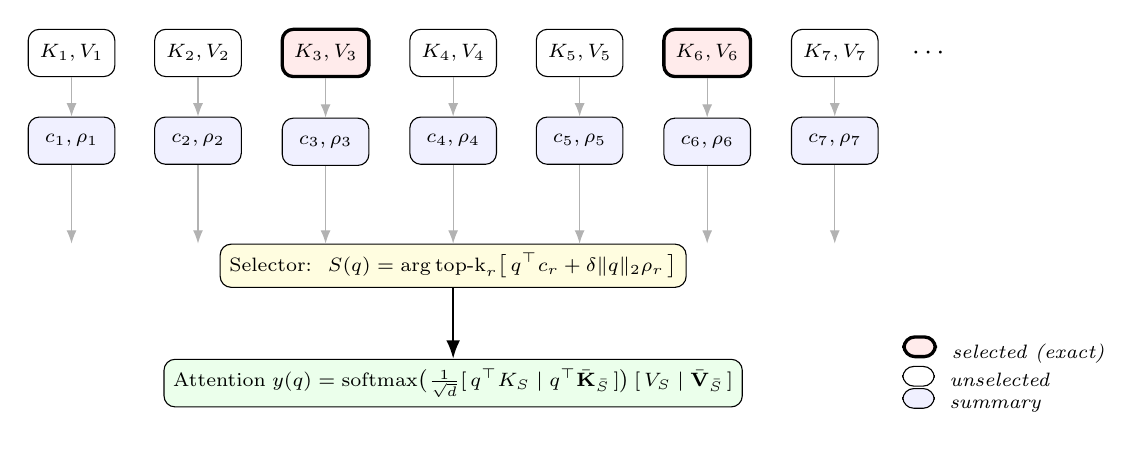
\begin{tikzpicture}[
  node distance=1.4em,
  block/.style={draw,rounded corners,minimum width=1.1cm,minimum height=0.6cm,font=\scriptsize,align=center,fill=white},
  summary/.style={draw,rounded corners,minimum width=1.1cm,minimum height=0.6cm,font=\scriptsize,align=center,fill=blue!6},
  selected/.style={draw,very thick,rounded corners,minimum width=1.1cm,minimum height=0.6cm,font=\scriptsize,align=center,fill=red!8},
  arrow/.style={-Latex,thick},
  note/.style={font=\scriptsize\itshape,align=center},
]

\node[block] (b1) {$K_1,V_1$};
\node[block,right=of b1] (b2) {$K_2,V_2$};
\node[selected,right=of b2] (b3) {$K_3,V_3$};
\node[block,right=of b3] (b4) {$K_4,V_4$};
\node[block,right=of b4] (b5) {$K_5,V_5$};
\node[selected,right=of b5] (b6) {$K_6,V_6$};
\node[block,right=of b6] (b7) {$K_7,V_7$};
\node[right=0.3cm of b7] (dots) {$\cdots$};

\node[summary,below=0.5cm of b1] (s1) {$c_1,\rho_1$};
\node[summary,below=0.5cm of b2] (s2) {$c_2,\rho_2$};
\node[summary,below=0.5cm of b3] (s3) {$c_3,\rho_3$};
\node[summary,below=0.5cm of b4] (s4) {$c_4,\rho_4$};
\node[summary,below=0.5cm of b5] (s5) {$c_5,\rho_5$};
\node[summary,below=0.5cm of b6] (s6) {$c_6,\rho_6$};
\node[summary,below=0.5cm of b7] (s7) {$c_7,\rho_7$};

\foreach \i in {1,...,7} {
  \draw[-Latex,gray!60,thin] (b\i.south) -- (s\i.north);
}

\node[draw,rounded corners,below=1.0cm of s4,fill=yellow!12,font=\scriptsize,align=center,minimum width=5.8cm] (sel) {Selector:\; $S(q) = \argtopk_r\bigl[\,q^\top c_r + \delta \normq \rho_r\,\bigr]$};

\foreach \i in {1,...,7} {
  \draw[-Latex,gray!60,thin] (s\i.south) -- (sel.north -| s\i.south);
}

\node[draw,rounded corners,below=0.9cm of sel,fill=green!8,font=\scriptsize,align=center,minimum width=7.1cm] (sm)
  {Attention\;$y(q) = \mathrm{softmax}\bigl(\tfrac{1}{\sqrt d}[\,q^\top K_{S} \;\vert\; q^\top \Kbar_{\bar S}\,]\bigr)\,[\,V_S \;\vert\; \Vbar_{\bar S}\,]$};

\draw[arrow] (sel.south) -- (sm.north);

\node[note,right=0.3cm of sm,xshift=1.6cm,align=left] {
  \tikz \node[selected,minimum width=0.4cm,minimum height=0.25cm] {}; \;selected (exact)\\
  \tikz \node[block,minimum width=0.4cm,minimum height=0.25cm] {}; \;unselected\\
  \tikz \node[summary,minimum width=0.4cm,minimum height=0.25cm] {}; \;summary \\
};

\end{tikzpicture}
\caption{\textbf{Method overview (Fig.~1).} The KV cache is partitioned
into fixed-size blocks. Each block carries a certified summary
$(c_r, \rho_r)$ with $\|k_j - c_r\|_2 \le \rho_r$ for every key
$k_j \in B_r$. A query scores all blocks via
$\ur(q) = q^\top c_r + \delta \normq \rho_r$ (Prop.~\ref{prop:cert}),
selects a small top-$k$ subset for exact token-level attention, and feeds
the rest as summaries in a single joint softmax.}
\label{fig:method}
\end{figure}

\subsection{Setup}

Let $n \in \N$ denote the KV-cache length at the point of attention and
$d \in \N$ the per-head hidden dimension. We partition the sequence axis
into $m = \lceil n / b \rceil$ fixed-size blocks of size $b$, padding the
final block by repeating its last entry. Formally, block $r \in \{1, \dots, m\}$
carries the token index set
\[
B_r \;=\; \bigl\{(r-1)b,\, (r-1)b + 1,\, \dots,\, \min(rb - 1,\, n - 1)\bigr\}
\]
and the corresponding key and value matrices $K_r \in \R^{b \times d}$,
$V_r \in \R^{b \times d}$. Let $k \in \N$, $k \ll m$, denote the
\emph{exact-attention budget} --- the maximum number of blocks whose
per-token keys and values will participate in the token-level softmax.
Grouped-query attention is handled by the standard repeat of KV heads
across query heads; the method is described per query head.

\subsection{Coarse-to-exact attention}
\label{sec:coarse-exact}

For each block $r$ we maintain a summary $(\bar k_r, \bar v_r) \in \R^{d} \times \R^{d}$,
taken as the per-head mean
\begin{equation}
\bar k_r \;=\; \frac{1}{|B_r|} \sum_{j \in B_r} k_j,
\qquad
\bar v_r \;=\; \frac{1}{|B_r|} \sum_{j \in B_r} v_j. \label{eq:summary}
\end{equation}
Given a query $q \in \R^{d}$ and a selection
$S(q) \subseteq \{1, \dots, m\}$ with $|S(q)| \le k$, the attention output is
\begin{equation}
y(q) \;=\; \mathrm{softmax}\!\left( \tfrac{1}{\sqrt d}\, \bigl[\,q^{\top} K_{S(q)} \,\bigm|\, q^{\top} \Kbar_{\bar S(q)}\,\bigr] \right) \cdot \bigl[\, V_{S(q)} \,\bigm|\, \Vbar_{\bar S(q)} \,\bigr], \label{eq:coarse-exact}
\end{equation}
where $K_{S(q)} \in \R^{|S| b \times d}$ is the row-concatenation of exact
token keys from the selected blocks, $V_{S(q)}$ the corresponding values,
and $\Kbar_{\bar S(q)} \in \R^{|\bar S| \times d}$, $\Vbar_{\bar S(q)}$
collect the summaries of the unselected blocks
$\bar S(q) = \{1,\dots,m\} \setminus S(q)$. We refer to the two halves of
this joint softmax as the \emph{exact-refine} and \emph{coarse} paths:
\begin{equation}
y(q) \;=\; \underbrace{y_{\mathrm{coarse}}(q)}_{\text{over }\{(\bar k_r, \bar v_r) : r \in \bar S\}} \;+\; \underbrace{y_{\mathrm{exact\text{-}refine}}(q)}_{\text{over }\{(k_j, v_j) : r \in S,\, j \in B_r\}}
\quad\text{(up to the shared softmax normaliser).}\label{eq:decomp}
\end{equation}
In practice we evaluate the joint softmax with a single fused kernel
call; the decomposition~\eqref{eq:decomp} is conceptual. Two invariants
matter: the exact KV cache is never discarded, so only the \emph{allocation}
of exact attention varies per query; and the softmax is causal and
well-defined for every query, including those whose selected blocks lie
entirely in the future.

\subsection{Certified block screening}
\label{sec:cert}

\begin{definition}[block summary with radius]
A \emph{certified block summary} for block $r$ is a pair
$(c_r, \rad) \in \R^{d} \times \R_{\ge 0}$ satisfying
\begin{equation}
\|k_j - c_r\|_2 \;\le\; \rad \quad \forall\, j \in B_r. \label{eq:radius-inv}
\end{equation}
\end{definition}

We take $c_r = \bar k_r$ from~\eqref{eq:summary} and
$\rad = \max_{j \in B_r} \|k_j - c_r\|_2$. Both are computed in bf16 with
fp32 accumulation of the squared distances:
\begin{equation}
\rad^2 \;=\; \max_{j \in B_r} \, \sum_{\ell=1}^{d} (k_{j,\ell} - c_{r,\ell})^2. \label{eq:rad-compute}
\end{equation}

\begin{proposition}[certified upper bound]
\label{prop:cert}
For every query $q \in \R^{d}$ and every key $k_j \in B_r$,
\begin{equation}
q^{\top} k_j \;\le\; q^{\top} c_r \,+\, \normq \rad \;=:\; \ur(q). \label{eq:bound}
\end{equation}
\end{proposition}

\begin{proof}
Write $q^{\top} k_j = q^{\top} c_r + q^{\top} (k_j - c_r)$. By
Cauchy--Schwarz, $|q^{\top}(k_j - c_r)| \le \normq \, \|k_j - c_r\|_2 \le \normq \rad$
using~\eqref{eq:radius-inv}. Therefore
$q^{\top} k_j \le q^{\top} c_r + \normq \rad = \ur(q)$. \qedhere
\end{proof}

Equation~\eqref{eq:bound} is a \emph{certified} bound: never violated by
construction. \S\ref{sec:tightness} reports the empirical violation
count (zero) and the slack statistic
$\text{slack}_r(q) = \ur(q) - \max_{j \in B_r} q^{\top} k_j \ge 0$.

\subsection{Selection policies}
\label{sec:selectors}

We compare two selection functions, both returning a $k$-subset of blocks.

\paragraph{FixedTopK.}
\begin{equation}
S_{\mathrm{fix}}(q) \;=\; \argtopk_r\bigl(q^{\top} c_r\bigr). \label{eq:fixed}
\end{equation}
Selection depends only on coarse summary scores. This is the natural
baseline selector and is closely related to per-page criticality scoring
in prior work.

\paragraph{BoundScreen.}
\begin{equation}
S_{\mathrm{bs}}(q; \delta) \;=\; \argtopk_r\bigl(q^{\top} c_r + \delta \cdot \normq \rad\bigr), \qquad \delta \in [0, 1]. \label{eq:boundscreen}
\end{equation}
At $\delta = 0$ this reduces to FixedTopK. At $\delta = 1$ selection ranks
blocks by the certified upper bound $\ur$ on their best possible
token-level score. We use $\delta = 1$ throughout unless otherwise noted.
The distinction is conceptually small but load-bearing: FixedTopK ranks
blocks by what is \emph{typical} inside them (the coarse dot product);
BoundScreen ranks blocks by what is \emph{possible} inside them (a
Cauchy--Schwarz upper bound on the best token-level score).

\subsection{Systems implementation}
\label{sec:systems}

Three design choices carry most of the performance story.

\paragraph{Shared-across-queries selection (gather\_shared).}
Within a single forward pass, all queries in a head share one selection $S$,
scored from the head's mean query
$\bar q = \frac{1}{L_q} \sum_{i=1}^{L_q} q_i$. The gathered key/value
tensors then have shape $(B, H_q, kb, d)$ --- no $L_q$ axis --- which
lets the post-gather attention use a single fused
\texttt{scaled\_dot\_product\_attention} call on a drastically reduced KV
set. Per-query causal masking is applied inside that single call, so
individual queries never attend to gathered tokens in their own future.
The alternative --- per-query selection and gather --- is bit-equivalent
to a masked reference implementation but runs approximately $12\times$
slower on the ROCm hardware we used, because \texttt{torch.gather} with
scattered reads along a large $L_q$ axis does not coalesce. We discuss
the retrieval consequences of this choice in \S\ref{sec:limitations}.

\paragraph{Residual-refine packing.}
Unselected-block summaries are concatenated onto the selected key/value
tensors as $m - k$ additional virtual tokens, giving a joint softmax of
size $kb + m - k$. This retains~\eqref{eq:decomp} without requiring a
separate forward pass, and keeps every query in causal contact with every
past block --- either via exact tokens from the selected blocks or via
a one-vector summary from each unselected one.

\paragraph{Radius caching.}
In the decode regime, each generation step extends the KV cache by one
token. All blocks' centres and radii except the last are unchanged; the
cache recomputes only the growing block:
\begin{equation}
(c_r^{(t+1)}, \rho_r^{(t+1)}) =
\begin{cases}
(c_r^{(t)}, \rho_r^{(t)}) & r < r^\star, \\
(\text{recomputed from } K_r^{(t+1)}, V_r^{(t+1)}) & r = r^\star,
\end{cases} \qquad r^\star = \bigl\lfloor \tfrac{n^{(t+1)} - 1}{b} \bigr\rfloor. \label{eq:radcache}
\end{equation}
This removes $O(n d)$ redundant work per decode step for the bound
selector, which is what lets BoundScreen's decode wall-clock catch up to
FixedTopK's despite carrying the extra radius computation.

\subsection{Complexity}
\label{sec:complexity}

Per query head, let $n$ be the KV length, $b$ the block size,
$m = \lceil n/b \rceil$ the block count, $k$ the exact budget, $d$ the
head dimension.

\begin{equation}
\text{per-query cost:}\qquad O\!\left(\underbrace{m d}_{\text{scoring}} + \underbrace{k b d}_{\text{exact-refine}}\right) = O\!\left(\!\left(\frac{n}{b} + k b\right) d\right), \label{eq:perquery-cost}
\end{equation}

\begin{equation}
\text{prefill cost ($n$ queries):}\qquad O\!\left(\frac{n^2 d}{b} + n k b d\right). \label{eq:prefill-cost}
\end{equation}
Prefill is \emph{reduced-quadratic}, not linear: the $n^2/b$ prefix
persists because each query still scores every past block. The ratio of
adaptive prefill to dense prefill $O(n^2 d)$ is
\begin{equation}
R(n, b, k) \;=\; \frac{n^2 d / b + n k b d}{n^2 d} \;=\; \frac{1}{b} + \frac{k b}{n}. \label{eq:ratio}
\end{equation}
At $b = 64$, $k = 6$, $n = 32\mathrm{k}$, $R \approx 0.028$ --- an
\emph{algorithmic ceiling}, not a speedup claim. It is what the method
could achieve if coarse scoring, gather, causal-mask construction, and
residual summary packing were free. The measured $5.30\times$ speedup at
$32\mathrm{k}$ in \S\ref{sec:latency} is what remains after those costs;
the gap between ceiling and measurement is concrete implementation surface,
not a theoretical loss.

Minimising $R$ over $b$ gives $b^{\star} = \sqrt{n/k}$ with
$R^{\star}(n, k) = 2\sqrt{k/n}$. For Qwen3-0.6B at $n = 32\mathrm{k}$,
$k = 6$, this yields $b^{\star} \approx 73$; the constraint
$b \in \{8, 16, 32, 64\}$ used elsewhere in the paper makes $b = 64$ the
nearest admissible value, which is what we use.

% ======================================================================
\section{Experimental Setup}
\label{sec:setup}
% ======================================================================

\paragraph{Model and runtime.}
All experiments use Qwen3-0.6B \citep{qwen3} (28 decoder layers,
$d_{\text{model}} = 1024$, 16 attention heads and 8 KV heads with
grouped-query attention, bf16). We do not fine-tune the model; adaptive
attention is applied as a drop-in replacement of the attention forward on
selected layers. The primary hardware is a single AMD Ryzen AI Max+~395
(Strix Halo, gfx1151) with 128\,GB unified memory, running PyTorch 2.10
with ROCm 7.2 and the experimental AOTriton SDPA kernels enabled
(\texttt{TORCH\_ROCM\_AOTRITON\_ENABLE\_EXPERIMENTAL=1}). Disabling that
flag places the baseline on a slow math fallback and inflates every
reported speedup by $\approx 3\times$; we report only numbers from the
fast-path configuration.

\paragraph{Methods compared.}
Three families throughout: \emph{dense baseline} (stock SDPA
\citep{dao2022flashattention}), \emph{FixedTopK} (Eq.~\ref{eq:fixed}),
and \emph{BoundScreen} (Eq.~\ref{eq:boundscreen}), all at $b = 64$ in
residual-refine mode. Exact-budget sweeps use $k \in \{4, 5, 6, 8\}$;
long-context latency sweeps focus on $k \in \{6, 8\}$.

\paragraph{Metrics.}
Prefill latency is reported as the median of $\ge 3$ timed iterations
(10 at context lengths up to $8\mathrm{k}$; 5 at $16\mathrm{k}$; 3 at
$32\mathrm{k}$ and $64\mathrm{k}$) following $\ge 3$ warm-up iterations in
the same process. Error bars ($\pm$) denote standard deviation within a
single session. Calibration perplexity is measured on a fixed
information-theory passage over non-overlapping 512-token windows:
\begin{equation}
\mathrm{PPL} \;=\; \exp\!\left( -\frac{1}{N - 1} \sum_{t=1}^{N - 1} \log p_\theta(x_{t+1} \mid x_{1:t}) \right).
\end{equation}
Passkey retrieval follows the standard needle-in-haystack
protocol \citep{liu2023lost} with a random 5-digit code injected at depth
$d \in \{0.1, 0.3, 0.5, 0.7, 0.9\}$ into a filler passage, scored by
teacher-forced greedy correctness over five seeds per cell.

\paragraph{Artifact protocol.}
Every table and figure in this paper is regenerated by a single script
from the JSON artifacts in \texttt{results/}. Where the same (method,
context length) cell appears in multiple bench files, we keep the sample
with the tightest within-session standard deviation. Source code, configs,
and raw result files are released with the paper.

% ======================================================================
\section{Main Results}
\label{sec:results}
% ======================================================================

\subsection{Long-context latency--quality tradeoff}
\label{sec:latency}

\begin{figure}[t]
\centering
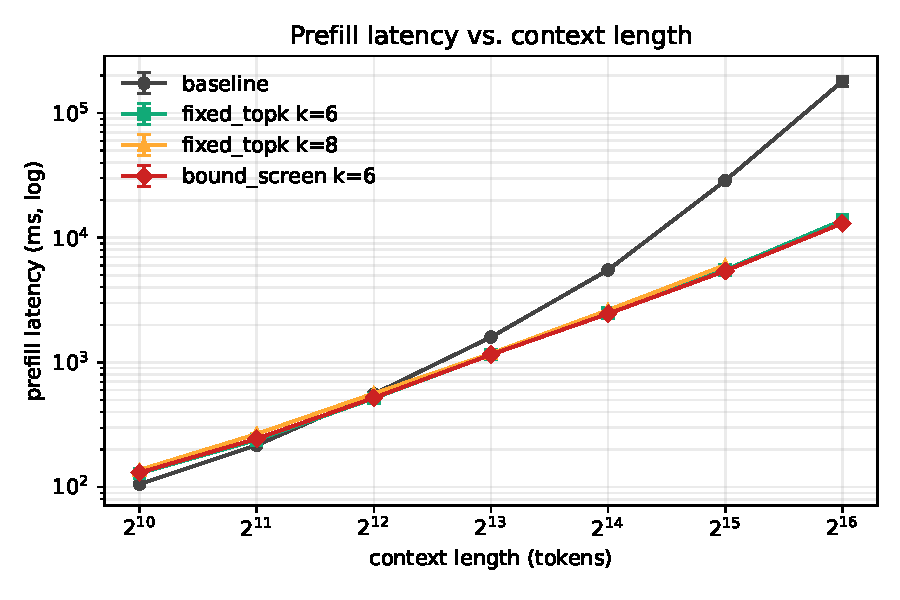
\includegraphics[width=0.80\linewidth]{figures/fig2_latency_vs_ctx.pdf}
\caption{\textbf{Prefill latency vs context length (Fig.~2).} Log--log.
Error bars are within-session standard deviations. BoundScreen at $k = 6$
crosses baseline between $2\mathrm{k}$ and $4\mathrm{k}$ and the gap
widens at longer context. The $65\mathrm{k}$ point exceeds Qwen3-0.6B's
training context and appears in the appendix only.}
\label{fig:latency}
\end{figure}

\begin{table}[t]
\centering
\small
\setlength{\tabcolsep}{5pt}
\begin{tabular}{rrrrrr}
\toprule
\textbf{ctx} & \textbf{baseline} & \textbf{FixedTopK $k{=}6$} & \textbf{FixedTopK $k{=}8$} & \textbf{BoundScreen $k{=}6$} & \textbf{speedup} \\
\midrule
1{,}024  & $105.9 \pm 2.3$    & $128.8 \pm 0.5$   & $137.6 \pm 0.8$   & $131.0 \pm 1.1$   & $0.81\times$ \\
2{,}048  & $216.9 \pm 3.8$    & $239.1 \pm 1.0$   & $267.0 \pm 0.8$   & $244.6 \pm 1.2$   & $0.89\times$ \\
4{,}096  & $558.8 \pm 4.3$    & $516.3 \pm 1.0$   & $564.0 \pm 2.0$   & $520.3 \pm 1.2$   & $\mathbf{1.07\times}$ \\
8{,}192  & $1596.0 \pm 11.2$  & $1155.6 \pm 1.6$  & $1178.6 \pm 2.1$  & $1154.1 \pm 3.2$  & $\mathbf{1.38\times}$ \\
16{,}384 & $5514.7 \pm 33.4$  & $2501.6 \pm 13.1$ & $2628.8 \pm 7.8$  & $2458.4 \pm 9.1$  & $\mathbf{2.24\times}$ \\
32{,}768 & $28703.0 \pm 563.5$ & $5517.6 \pm 10.4$ & $6027.4 \pm 11.6$ & $5415.4 \pm 14.6$ & $\mathbf{5.30\times}$ \\
\bottomrule
\end{tabular}
\caption{\textbf{Prefill latency vs context length (Table~1).} Milliseconds; median $\pm$ within-session standard deviation. Bold rows mark BoundScreen outperforming the dense baseline. The $65{,}536$ row appears in the appendix because it exceeds Qwen3's training context.}
\label{tab:latency}
\end{table}

Define the empirical speedup at context length $n$ as
\begin{equation}
\mathrm{Speedup}(n) \;=\; \frac{T_{\mathrm{baseline}}(n)}{T_{\mathrm{BoundScreen}}(n)}.
\end{equation}
Results are given in Table~\ref{tab:latency} and Figure~\ref{fig:latency}.
The headline row is BoundScreen at $k = 6$:
\[
\mathrm{Speedup}(4\mathrm{k}) = 1.07\times, \;\;
\mathrm{Speedup}(8\mathrm{k}) = 1.38\times, \;\;
\mathrm{Speedup}(16\mathrm{k}) = 2.24\times, \;\;
\mathrm{Speedup}(32\mathrm{k}) = 5.30\times.
\]
Crossover against the dense baseline occurs between $2\mathrm{k}$ and
$4\mathrm{k}$: below it, the coarse-score computation and mask bookkeeping
dominate; above it, the $O(n^2/b)$ scaling of coarse scoring pulls ahead
of dense $O(n^2)$ attention, and the gap widens at the rate predicted by
\eqref{eq:ratio}. At $32\mathrm{k}$, a $28.7$\,s dense prefill collapses
to $5.4$\,s.

Calibration perplexity is preserved. The Qwen3-0.6B baseline PPL is
$11.096$; BoundScreen at $k = 6$ measures $11.105$, and FixedTopK at
$k = 8$ measures $11.113$. These differences sit well within run-to-run
jitter on a single-passage calibration metric; we describe them as ``no
measurable loss,'' not as an improvement.

Intra-session variance is small: standard deviations are under $15$\,ms
at every length up to $32\mathrm{k}$ (about $0.5\,\%$ of the median at
$32\mathrm{k}$). The one exception is the $64\mathrm{k}$ baseline, whose
large standard deviation reflects the position-embedding regime rather
than the measurement protocol; we omit that row from quality-bearing
claims.

\subsection{Graceful degradation under tight exact budgets}
\label{sec:degradation}

\begin{figure}[t]
\centering
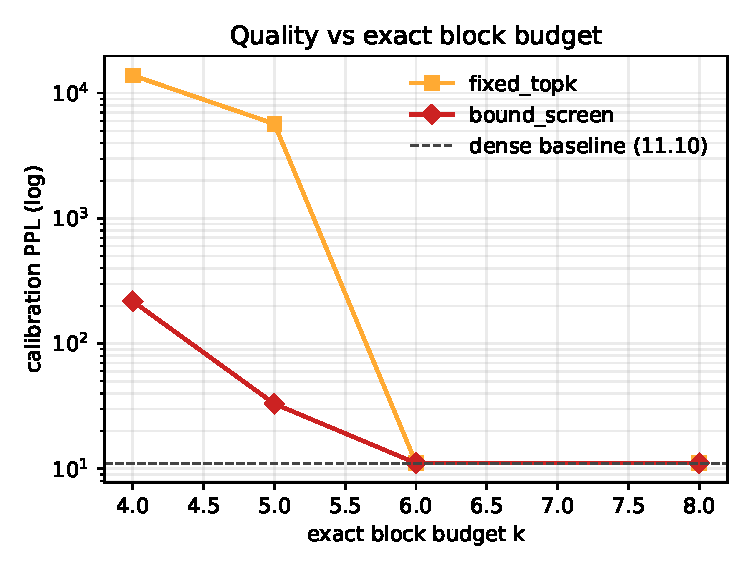
\includegraphics[width=0.72\linewidth]{figures/fig3_ppl_vs_k.pdf}
\caption{\textbf{Calibration perplexity vs exact budget (Fig.~3).}
Log-$y$. Both selectors meet baseline at $k \ge 6$. Below that, FixedTopK
degrades catastrophically; BoundScreen degrades, but by roughly two orders
of magnitude less at $k = 4$.}
\label{fig:degradation}
\end{figure}

\begin{table}[t]
\centering
\small
\begin{tabular}{r r r}
\toprule
$k$ & \textbf{FixedTopK PPL} & \textbf{BoundScreen PPL} \\
\midrule
4 & $13{,}865$ & $217.8$ \\
5 & $5{,}689$  & $33.042$ \\
6 & $11.113$   & $11.105$ \\
8 & $11.113$   & $11.086$ \\
\bottomrule
\end{tabular}
\caption{\textbf{PPL vs exact block budget (Table~2).} Block size $64$, residual-refine. Baseline PPL $= 11.096$. Contribution: graceful degradation at $k \le 5$, not lower budget at iso-quality.}
\label{tab:degradation}
\end{table}

Table~\ref{tab:degradation} and Figure~\ref{fig:degradation} summarise the
quality-vs-budget behaviour at $b = 64$. Both selectors meet baseline
calibration perplexity at $k \ge 6$; the contribution is below that
operating point.

At $k = 5$, FixedTopK loses three orders of magnitude of perplexity
($11 \to 5{,}689$); BoundScreen loses less than one ($11 \to 33$). At
$k = 4$, FixedTopK reaches $\approx 10^4$ while BoundScreen is two orders
of magnitude lower. Quantitatively, the log-PPL gap between selectors at
matched budget is
\begin{equation}
\log_{10} \frac{\mathrm{PPL}_{\mathrm{FixedTopK}}}{\mathrm{PPL}_{\mathrm{BoundScreen}}} \;\approx\;
\begin{cases}
1.80 & k = 4, \\
2.24 & k = 5.
\end{cases}
\end{equation}
Neither selector is usable at $k \le 5$ in the strict sense --- both fall
below any reasonable quality floor --- but the \emph{failure mode} is
qualitatively different: FixedTopK drops off a cliff, BoundScreen
degrades.

We frame the contribution as a change of failure mode, not as
lower-budget behaviour at matched quality. At the operating point where
an exact budget is provisioned conservatively enough to be correct on its
headline workload, both selectors work. Under provisioning error ---
a shorter budget than expected, a workload with less average-case
redundancy than expected --- BoundScreen continues to produce coherent
output at perplexities that are two orders of magnitude better than the
coarse-ranking alternative. This is the behaviour the bound is designed
to deliver: a block whose best possible token-level score is large is
never silently dropped simply because its average score is unremarkable.

\subsection{Bound behaviour and selector restructuring}
\label{sec:tightness}

\begin{figure}[t]
\centering
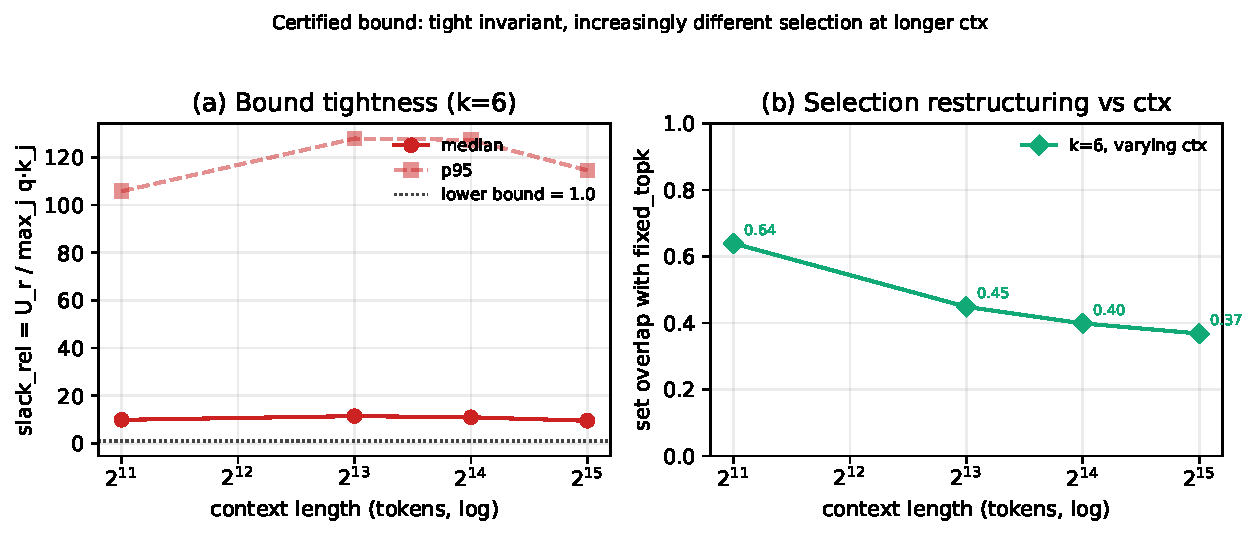
\includegraphics[width=0.88\linewidth]{figures/fig4_tightness_and_overlap.pdf}
\caption{\textbf{Bound tightness and selection restructuring (Fig.~4).}
(a) Median and $p95$ of $\ur(q) / \max_j q^{\top} k_j$ across probed
queries; always $\ge 1$ by Prop.~\ref{prop:cert}, and stable around $10$
across context lengths. (b) Set overlap between BoundScreen and FixedTopK
selected blocks at $k = 6$; divergence grows with context length,
reaching $0.37$ at $32\mathrm{k}$.}
\label{fig:tightness}
\end{figure}

\begin{definition}[bound slack]
For a query $q$ and block $r$, define
\begin{equation}
\mathrm{slack}_r(q) \;=\; \ur(q) - \max_{j \in B_r} q^{\top} k_j \;\ge\; 0, \qquad
\mathrm{slack\text{-}rel}_r(q) \;=\; \frac{\ur(q)}{\max_{j \in B_r} q^{\top} k_j} \;\ge\; 1.
\end{equation}
\end{definition}

\begin{definition}[selection overlap]
For selectors $S_1, S_2$ at the same budget $k$,
\begin{equation}
\mathrm{overlap}_k(q) \;=\; \frac{|S_1(q) \cap S_2(q)|}{k} \;\in\; [0, 1].
\end{equation}
We report the mean over probed queries and blocks.
\end{definition}

\paragraph{Violations and slack.}
For every $(q, r)$ pair probed, Proposition~\ref{prop:cert} requires
$\mathrm{slack\text{-}rel}_r(q) \ge 1$. Across every probed configuration
--- context lengths $2\mathrm{k}$, $8\mathrm{k}$, $16\mathrm{k}$, $32\mathrm{k}$
at $k = 6$, plus $k \in \{4, 8\}$ at $2\mathrm{k}$ --- the ratio is
$\ge 1$ on every sampled cell: zero observed violations
(Figure~\ref{fig:tightness}a). The median ratio stays in the $9.5$--$10.9$
range across all contexts, indicating that the bound is loose in absolute
terms (roughly an order of magnitude above the actual block-max logit)
but remarkably stable. Slack does not widen with context length,
consistent with the derivation of \eqref{eq:bound} having no $n$-dependence.

\paragraph{Restructuring vs FixedTopK.}
Figure~\ref{fig:tightness}b plots $\mathrm{overlap}_6$ between
BoundScreen and FixedTopK as context grows: $0.64$ at $2\mathrm{k}$,
$0.45$ at $8\mathrm{k}$, $0.40$ at $16\mathrm{k}$, $0.37$ at $32\mathrm{k}$.
By $32\mathrm{k}$, $63\,\%$ of BoundScreen's six selected blocks are not
in FixedTopK's top-6. This rules out the interpretation that BoundScreen
is a relabelling of FixedTopK: the two selectors make measurably different
picks at long context. \S\ref{sec:degradation} is a separate experiment
--- different $k$, different context --- but shows that the selectors'
behaviours also differ under tight exact budgets, in the direction the
bound would predict. We do not directly attribute the graceful
degradation to the specific picks the overlap measurement identifies; we
state only that (i) the two selectors are empirically distinct and (ii)
BoundScreen is the one that preserves graceful degradation.

% ======================================================================
\section{Limitation Analysis}
\label{sec:limitations}
% ======================================================================

\subsection{Passkey retrieval failure at $b = 64$}
\label{sec:passkey}

\begin{figure}[t]
\centering
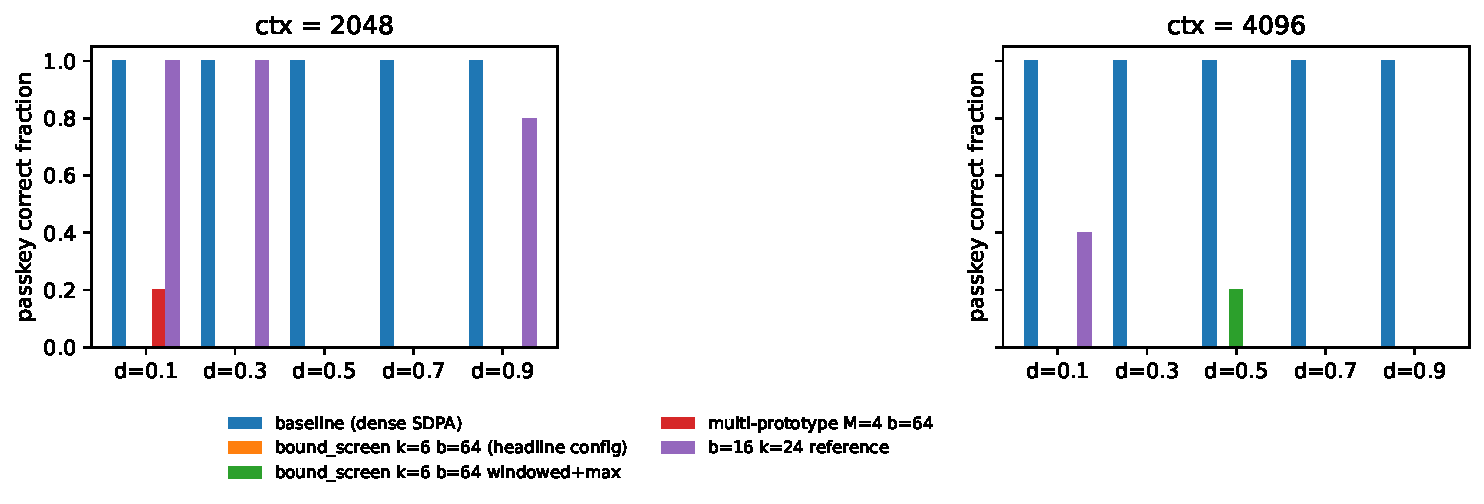
\includegraphics[width=0.95\linewidth]{figures/fig5_passkey.pdf}
\caption{\textbf{Passkey retrieval correctness by depth (Fig.~5)}, at
$2\mathrm{k}$ and $4\mathrm{k}$ context. Baseline is dense SDPA. All
$b=64$ adaptive variants are at or near zero across all depths. The
$b = 16$ reference recovers retrieval at easy depths only; the mechanism
is analysed in \S\ref{sec:passkey-mechanism}.}
\label{fig:passkey}
\end{figure}

We probe sparse single-token retrieval with a standard passkey test
\citep{liu2023lost}: a 5-digit magic number is injected at depth
$d \in \{0.1, 0.3, 0.5, 0.7, 0.9\}$ into a filler passage of context
length $n \in \{2048, 4096\}$, and a trailing query ``what is the magic
number? A:'' elicits a teacher-forced completion. Correctness is the
fraction of trials (over five seeds) whose greedy completion matches
the injected digits token-by-token. Results appear in
Figure~\ref{fig:passkey}.

The dense SDPA baseline scores $1.00$ at every (context, depth) cell.
Every adaptive variant at $b = 64$ scores at or near zero. BoundScreen at
$k = 6$ with shared-mean selection: zero across every cell. BoundScreen
with windowed-max aggregation (a per-query-window variant): zero except a
single $0.20$ cell at $4\mathrm{k}/d = 0.5$. BoundScreen with $\delta = 5$
(radius-term-dominant selection): zero. A reference configuration at
$b = 16, k = 24$ --- using the same gather budget in tokens
($k b = 384$) but a finer block partition --- recovers $1.00$ correctness
at $d = 0.1$ and $0.80$ at $d = 0.9$, but still fails at mid-depth.

We state this plainly: the method as built is not a general retrieval
architecture. The pattern of failure is not a selector tuning artefact.

\subsection{Mechanism}
\label{sec:passkey-mechanism}

The failure has two mechanisms that compound.

\paragraph{Summary dilution.}
Consider a block whose keys are one informative \emph{needle} key $k^\star$
plus $b - 1$ filler keys $\{k_j\}$, and write
$\mathbb{E}[k_j] = \mu$, $\mathrm{Var}[k_j] = \sigma^2$ for the filler
distribution. The mean summary is
\begin{equation}
c_r \;=\; \frac{1}{b}\left(k^\star + \sum_{j \ne j^\star} k_j\right) \;\approx\; \mu + \frac{k^\star - \mu}{b},
\end{equation}
so the needle contributes $O(1/b)$ to the center direction. For a query
$q$ whose retrieval signal lies in the $k^\star - \mu$ direction, the
coarse-score gap between the needle block and a pure-filler block is
$O(1/b)$. At $b = 64$ this is small enough that the query's coarse-score
ordering is dominated by filler-direction noise rather than by the
needle contribution. The radius term $\normq \rad$ in \eqref{eq:bound}
does grow when the block contains an outlier --- but for retrieval
queries at this model scale, $q^{\top} c_r$ dominates the ranking.
Raising $\delta$ to 5 (radius-term-dominant selection) does not rescue
this: the invariant \eqref{eq:radius-inv} still holds, but the radius
term alone is not discriminative enough to distinguish a needle block
from its neighbours.

\paragraph{Selection granularity.}
A 64-token block is the unit of selection. Keeping it requires
outscoring $31$ other blocks at $2\mathrm{k}$ with six picks. At $b = 16$
the same argument operates against $127$ blocks with $24$ picks --- a
four-times-larger selection budget at four-times-finer granularity ---
and a $1/16$ dilution is more often distinguishable from a $0/16$ filler
block than $1/64$ is from $0/64$. The $b = 16$ reference in
\S\ref{sec:passkey} recovers retrieval at easy depths under exactly this
accounting.

Neither mechanism alone is decisive; together they are.

\subsection{Negative result: multi-prototype}
\label{sec:multiproto}

A natural fix is to split each block into $M$ sub-blocks, store one
$(c_{r,m}, \rho_{r,m})$ pair per sub-block, and bound the block via
\begin{equation}
\ur^{(M)}(q) \;=\; \max_{m=1,\dots,M} \bigl(q^{\top} c_{r,m} + \normq \rho_{r,m}\bigr). \label{eq:mp-bound}
\end{equation}
This remains a certified upper bound: the pointwise max of upper bounds
is an upper bound on the pointwise max. Formally, for $j \in B_{r,m}$,
\[
q^{\top} k_j \;\overset{\text{Prop.~\ref{prop:cert}}}{\le}\; q^{\top} c_{r,m} + \normq \rho_{r,m} \;\le\; \max_{m'} \bigl(q^{\top} c_{r,m'} + \normq \rho_{r,m'}\bigr) = \ur^{(M)}(q),
\]
so $\max_{j \in B_r} q^{\top} k_j \le \ur^{(M)}(q)$.
We implemented \eqref{eq:mp-bound} for $M \in \{2, 4, 8\}$ with equal
sub-block splits and verified the invariant holds in every probe.

\begin{table}[t]
\centering
\small
\begin{tabular}{r r r r r}
\toprule
$M$ & passkey cells $>0$ & best cell & PPL & $8\mathrm{k}$ prefill \\
\midrule
1 & 0 / 10  &  0\,\%   & 11.082 & 2{,}210 ms \\
2 & 0 / 10  &  0\,\%   & 11.114 & 3{,}374 ms \\
4 & 1 / 10  & 20\,\%   & 11.084 & 4{,}624 ms \\
8 & 0 / 10  &  0\,\%   &  ---    &   ---     \\
\midrule
$b = 16, k = 24, M = 1$ (ref.) & 6 / 10 & 100\,\% & 11.110 & 4{,}572 ms \\
\bottomrule
\end{tabular}
\caption{\textbf{Multi-prototype at $b = 64, k = 6$ (Table~3)}, residual-refine, windowed max, compared to a fine-block reference. Retrieval does not improve; latency regresses monotonically with $M$. Calibration perplexity is preserved throughout.}
\label{tab:multiproto}
\end{table}

Table~\ref{tab:multiproto} shows that retrieval is not restored and that
latency regresses monotonically with $M$: the $M$-fold increase in
scoring cost is not amortised by any reduction in the downstream
attention shape, which still sees $kb + m$ keys. Calibration PPL is
preserved, consistent with multi-prototype leaving average-case modelling
behaviour intact.

\paragraph{The precise lesson: summary resolution alone is insufficient
when selection granularity stays coarse.} Multi-prototype gives each
block $M$ (center, radius) pairs, so per-prototype summaries cover
$b/M$ tokens --- as distinctive as a finer block would produce. But the
selector still picks $k$ blocks out of $m$, not $kM$ prototypes out of
$mM$. The passkey needs finer selection as well as finer summaries. Any
fix that recovers selection resolution by treating each prototype as a
selectable unit collapses to ``use block size $b/M$'' and pays the
$\lceil n/(b/M) \rceil$ summary count in the softmax key set --- which
is the latency cost we saw in the $b = 16$ reference row.

\subsection{Interpretation}
\label{sec:interpretation}

The method is effective for long-context inference under calibration/PPL-style
objectives: the selector preserves average modelling behaviour, the bound
gives real graceful degradation under under-provisioned exact budgets,
and the systems implementation delivers growing wall-clock wins at longer
contexts. It is \emph{not} a mechanism for retrieving sparse single-token
information at the coarse block granularities tested here.

The correct positioning is the framing sentence: this is a certified
runtime screening method for long-context efficiency, not a general
retrieval architecture. Quest \citep{tang2024quest} and our method use
different per-block metadata with different tradeoffs: Quest maintains
per-page element-wise key min/max ($2d$ scalars per block) and scores
against those min/max bounds --- finer-grained per-token information at
the cost of more scoring operations; we store one center and one scalar
radius ($d + 1$ scalars) and derive our bound from Cauchy--Schwarz
--- coarser metadata and a cheaper scoring pass, but a provable
block-level upper bound in one line. Neither design point dominates the
other; architectures such as DuoAttention \citep{xiao2024duoattention},
which separate retrieval heads from streaming heads, suggest that a
production system wanting both sparse-retrieval fidelity and the present
method's long-context wall-clock behaviour would likely compose them.

% ======================================================================
\section{Discussion}
% ======================================================================

\paragraph{Where the method is useful.}
Long-context prefill of existing dense pretrained models at context
lengths of $\sim 4\mathrm{k}$ and above, where the $O(n^2/b)$ scaling of
coarse scoring comfortably beats dense $O(n^2)$ attention;
runtime-efficient approximate exact attention for latency-sensitive
long-context inference; scenarios where average-modelling behaviour and
graceful degradation under tight budgets matter more than pinpoint
single-token retrieval.

\paragraph{Where it is not the right tool.}
Tasks that require recovering a specific distant token with high
probability --- passkey retrieval \citep{liu2023lost}, exact code-span
lookup, fact extraction from long documents --- at least at the 64-token
block granularity used here. Applications of this kind warrant
finer-grained per-page metadata along the lines Quest
\citep{tang2024quest} uses, or a dedicated retrieval mechanism
orthogonal to the present work.

\paragraph{Future directions.}
Finer selection granularity without the residual summary cost (e.g.\
hierarchical selection, or decoupling summary granularity from gather
granularity); tighter bounds than the isotropic Cauchy--Schwarz form
(axis-aligned box bounds along the lines of Quest's per-dimension
metadata, Mahalanobis-style whitening); hybrid stacks that apply
certified screening only to layers where it helps and dense attention
elsewhere, analogous to head-level routing in DuoAttention
\citep{xiao2024duoattention}. We explicitly do not speculate on
fine-tuning the selector; every result in this paper is from a single
frozen dense model.

% ======================================================================
\section{Conclusion}
% ======================================================================

We showed that certified block screening enables a practical adaptive
long-context attention mechanism with strong wall-clock gains at context
lengths of $4\mathrm{k}$ and above, reaching a $5.30\times$ prefill
speedup over a dense SDPA \citep{dao2022flashattention} baseline at
$32\mathrm{k}$ tokens on Qwen3-0.6B \citep{qwen3} while preserving
calibration perplexity and improving under-budget robustness. We also
identified a clear limitation: coarse block screening at 64-token
granularity does not recover sparse single-token retrieval, and simple
multi-prototype extensions fail to rescue retrieval because selection
granularity, not summary granularity, is the limiting factor. These
results position certified block screening as a useful runtime efficiency
tool rather than a universal replacement for exact long-range retrieval.

\bibliographystyle{plainnat}
\bibliography{references}

\end{document}
